Symbol definition:
\begin{center}
\begin{tabular}{|r|p{8cm}|}
\hline
$ p_0 $ & In the cure range, the maximum dosage required to
cure each Ebola patient.\\
\hline
$ Q(t) $ & The amount of drug at time $t$.\\
\hline
\end{tabular}
\end{center}%
Assumptions:
\begin{enumerate}
  \item The Ebola virus has no variation in the present period.
\end{enumerate}
The amount of the drug required to $ Q(t)=p_0*i(t) $.\par
The figure for $ i(t) $ in Case 2 shown as below:
\begin{center}
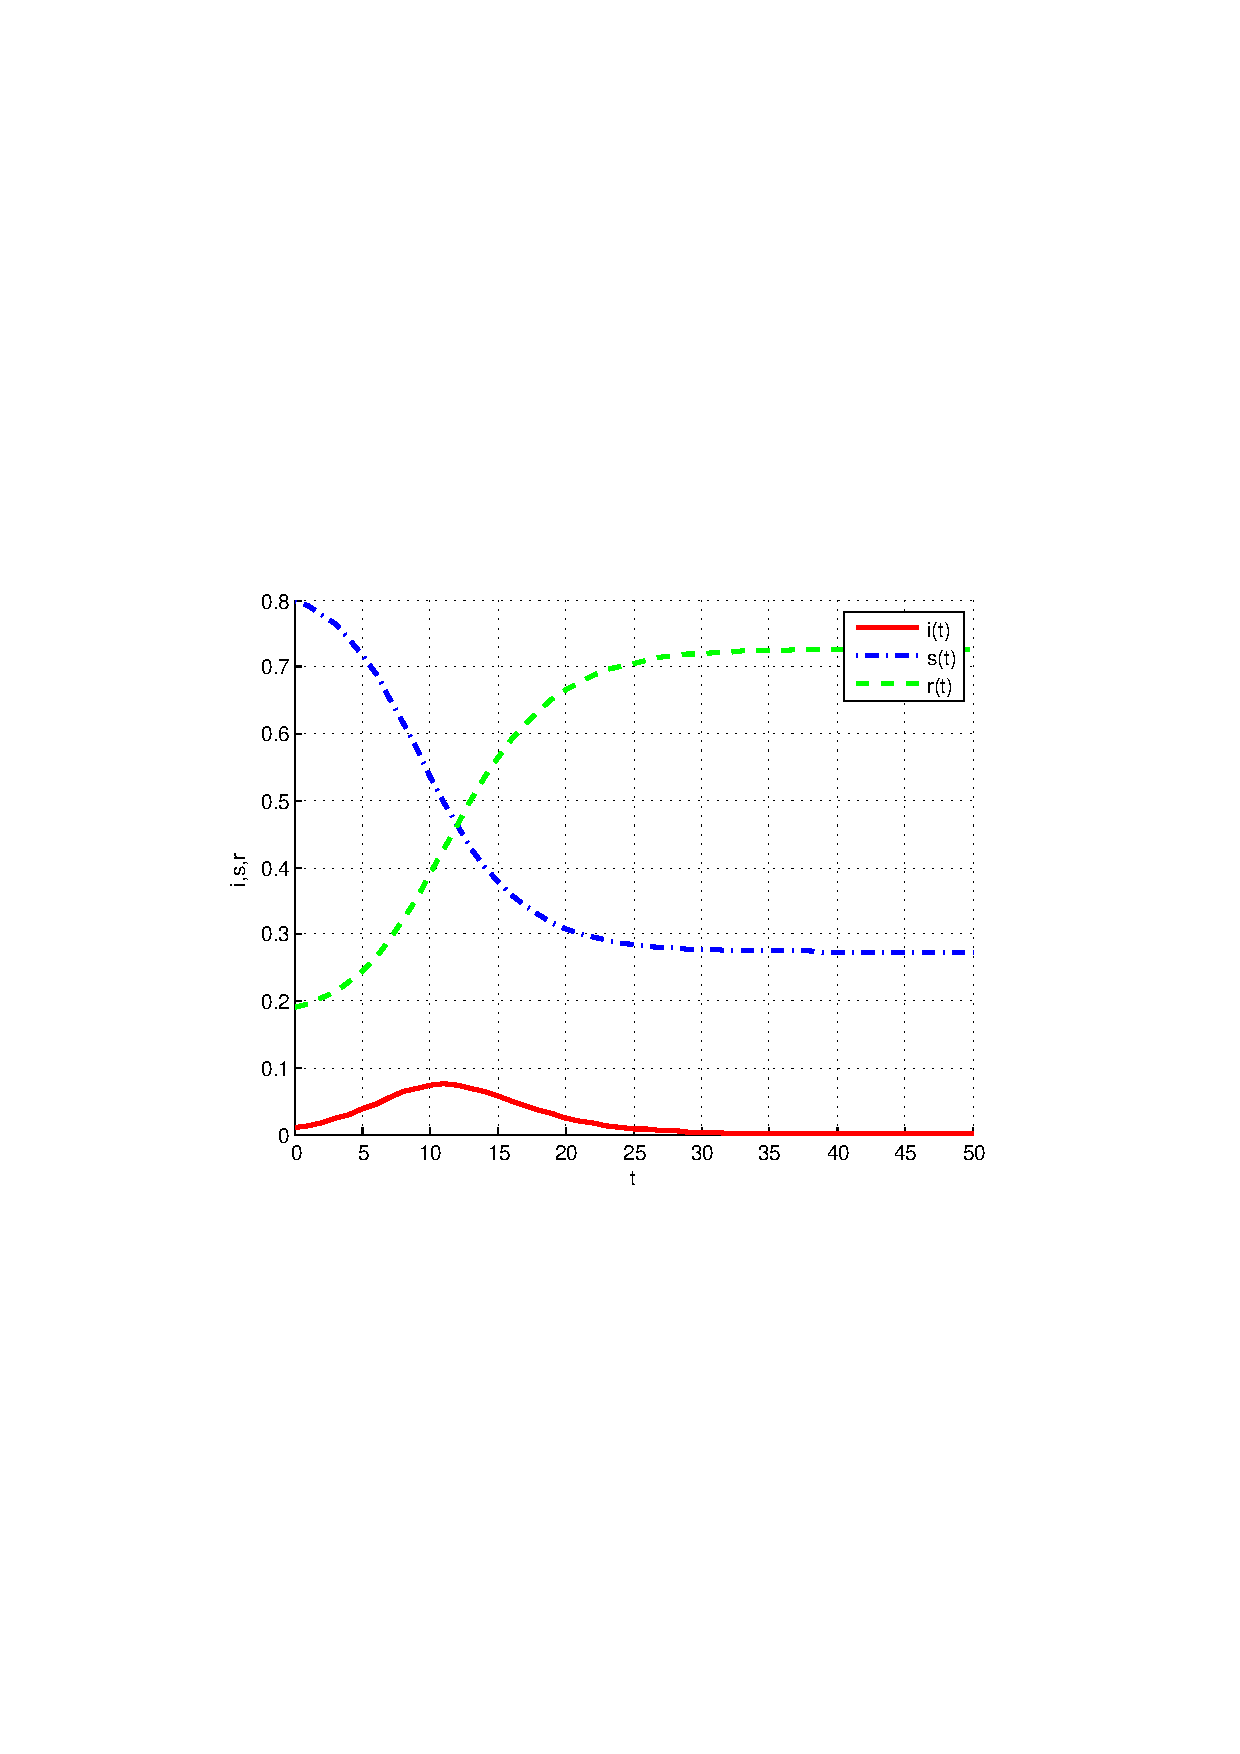
\includegraphics[width=4in]{imgs/sars3_1.pdf}
\end{center}
The amount of drug $Q(t)$ can be calculated is $p_0$ times of
$i(t)$, $Q(t)$ change with $t$ similar to $i$ change with $t$.
